\section{Einführung Wasserfarben}
Die moderne Form der Malerei mit Wasserfarben erlangte Ende des 18.\ 
Jahrhunderts ihre breite Anerkennung. Mithilfe von Wasserfarben lassen sich die 
unterschiedlichsten Effekte und Strukturen erzielen, die beispielsweise durch 
das Wandern der im Wasser gelösten Farbpigmente über das Papier entstehen. In 
den nächsten Abschnitten sollen die grundlegenden hierzu verwendeten 
Materialien und Techniken kurz vorgestellt werden.

\subsection{Materialien}
Das bei der Wasserfarbenmalerei verwendete \textbf{Papier} ist zumeist nicht 
wie üblich aus Zellstoff (also z.\,B.\ Baumholz), sondern aus Leinen oder 
Baumwolle hergestellt. Das Papier erhält durch die netzartige Struktur sein 
charakteristisches, unebenes Erscheinungsbild. Zur Imprägnierung des Papiers 
wird Zellulose benutzt, welche die Fasern umhüllt und einige der Poren 
ausfüllt. Auf diese Weise kann Wasser nicht mehr völlig ungehindert absorbiert 
werden - die Struktur bleibt trotzdem erhalten.

Die eigentliche \textbf{Wasserfarbe} besteht aus in Wasser gelösten Pigmenten,
einem Bindemittel sowie einem Tensid (oberflächenaktiver Stoff). Pigmente
bestehen aus einzelnen festen Partikeln und werden typischerweise zu einem Puder
verarbeitet. Sie können in das Papier eindringen und sich mithilfe des
Bindemittels anhaften. Pigmente unterscheiden sich in ihrer Dichte - eine hohe
Dichte sorgt dafür, dass sich das Pigment im Wasser nicht sehr weit bewegen
kann, bei geringer Dichte können die Partikel weiter "`wandern"'.
Das Tensid dient dazu, die Oberflächenspannung des Papiers herabzusetzen und es
dem Wasser so zu ermöglichen, in das Papier einzudringen und es zu durchtränken.

\subsection{Techniken}
Es werden hauptsächlich zwei Pinseltechniken verwendet. Zum einen das sog.\ 
\textsl{wet-on-wet}-, zum anderen das \textsl{wet-on-dry}-painting. Bei der
ersten Maltechnik wird mit einem nassen und farbgetränkten Pinsel auf bereits
nassem Papier gemalt. Auf diese Weise kann sich das Wasser und somit die Farbe
frei verteilen. Beim \textsl{wet-on-dry}-painting hingegen wird auf trockenem
Papier gemalt. Beide Techniken erzeugen die für die Wasserfarbenmalerei
charakteristische Effekte, welche im nächsten Abschnitt vorgestellt werden
sollen.

\subsection{Effekte}
Durch das Zusammenspiel von Wasserverlauf, Papierstruktur und Pigmentdichte 
können bei der Wasserfarbenmalerei die verschiedensten Effekte erzielt werden. 
In Abbildung \ref{fig:effects-real} sind die wichtigsten dieser Effekte 
aufgeführt.

\begin{figure}
  \centering
  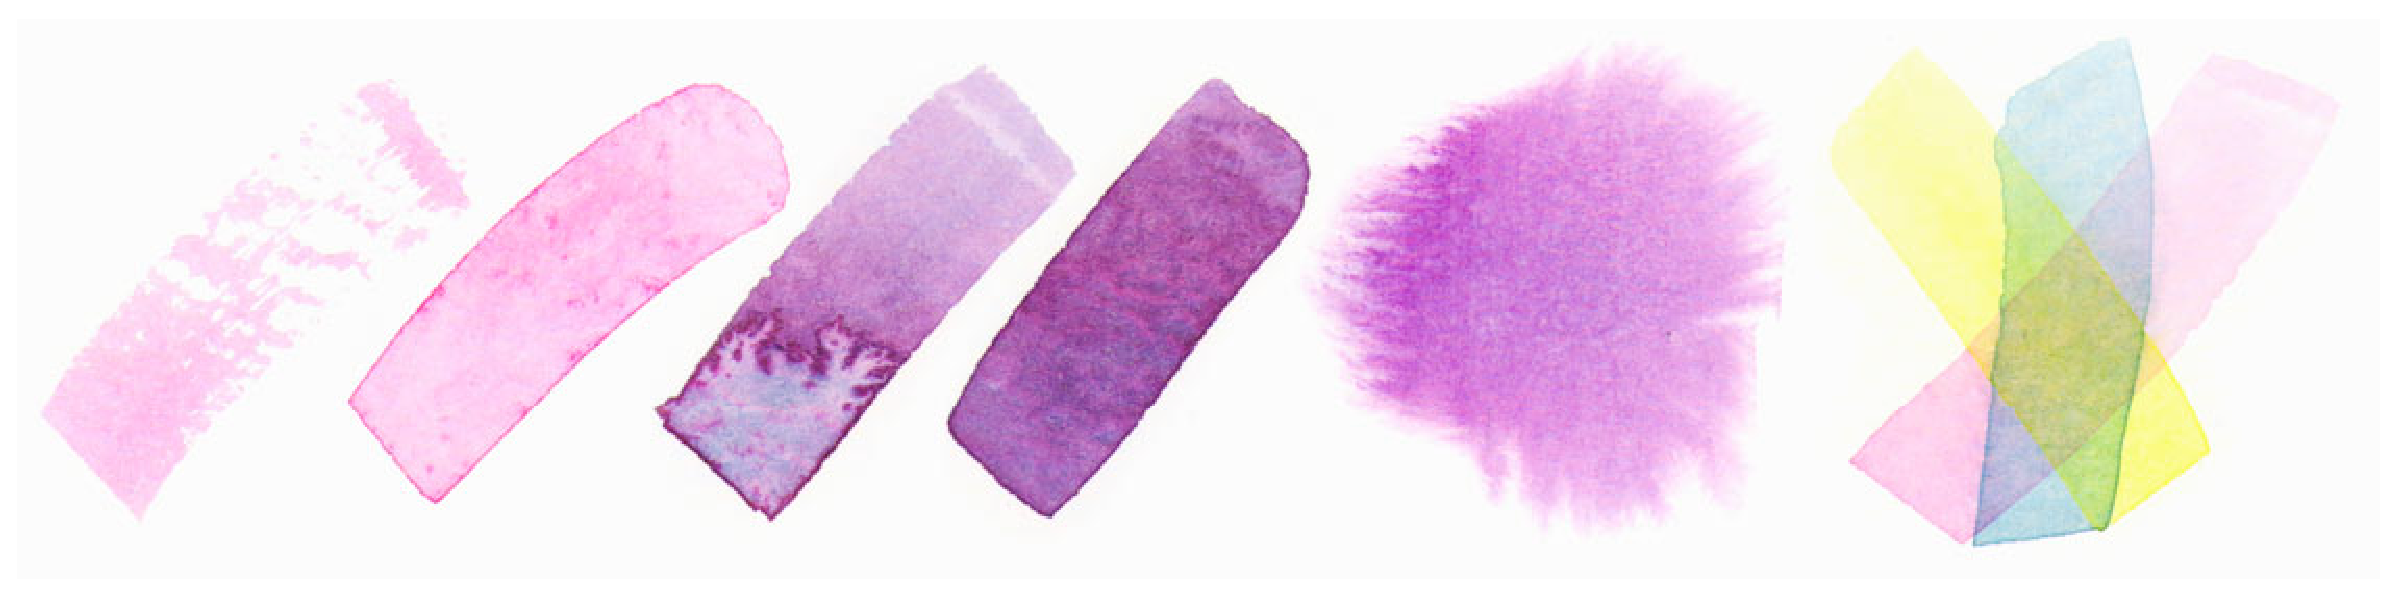
\includegraphics[width=1.00\textwidth]{../images/Curtis1997-real-watercolor-effects.eps}
  \caption{Wasserfarbeneffekte v.l.n.r.: drybrush, edge darkening, backrun,
  granulation, flow effect, glazing. Quelle: \cite{Curtis1997}.}
  \label{fig:effects-real}
\end{figure}

Bei der Verwendung der \textsl{wet-on-wet}-Pinseltechnik können die folgenden
Effekte entstehen:

\begin{itemize}
  \item \textsl{backrun}: Tritt auf, wenn eine Wasserlache zurück in eine
  feuchte Region fließt und das Wasser auf diese Weise Pigmente weiter verteilt.
  Es entstehen komplexe, verzweigte Formen mit teilweise dunklen Kanten.
  \item \textsl{ganulation}, \textsl{separation}: Die Granulierung der Pigmente
  ergibt eine körnige Textur, welche die Spitzen und Täler des Papiers betont.
  Je nach Pigment fällt die Granulierung natürlich anders aus und der Effekt
  kommt am stärksten bei sehr nassem Papier zum tragen. \textsl{Separation}
  bedeutet, dass unterschiedlich dichten Pigmente verschieden weit transportiert
  werden und somit eine Trennung der Farben entsteht.
  \item \textsl{flow pattern}: Die nasse Oberfläche des Papiers ermöglicht, dass
  der Pinselstrich sich frei ausbreitet und weiche, federartige Formen erzeugt
  werden. 
\end{itemize}

Die folgenden Effekte werden mithilfe der \textsl{wet-on-dry}-Technik erzeugt:

\begin{itemize}
  \item \textsl{dry brush}: Wird der trockene Pinsel im richtigen Winkel
  angewandt, so werden nur die erhabenen Stellen des Papiers mit Farbe bedeckt.
  Darus entstehen unregelmäßige Lücken mit ausgefransten Kanten.
  \item \textsl{edge darkening}: Während des Trockenvorgangs wandern die 
  Pigmente aus dem inneren des Pinselstrichs nach außen. Auf diese Weise 
  entstehen dunkle Schattierungen an den Kanten.
  \item \textsl{glazing}: Werden mehrere, dünne Farbschichten nach dem Trocknen
  übereinander gemalt, sodass die einzelnen Farbschichten optisch gemischt werden.
\end{itemize}

\section{Computer-erzeugte Wasserfarben}
Bei der Simulation von Wasserfarben kommt es nach \cite{Curtis1997} darauf an, 
nicht nur die physikalischen Eigenschaften des Mediums zu berücksichtigen, 
sondern auch die für diese Maltechnik charakteristischen Phänomene - nur wenn 
diese realistisch wiedergegeben werden können, ist die Simulation gelungen.

\subsection{Simulation}
In den folgenden Kapiteln wird die Simulation von Wasserfarben nach
\cite{Curtis1997} mit ihren einzelnen Teilbereichen näher beschrieben. Abbildung
\ref{fig:effects-simulated} zeigt die Ergebnisse der Simulation anhand der
bereits vorgestellten Effekte.

\begin{figure}
  \centering
  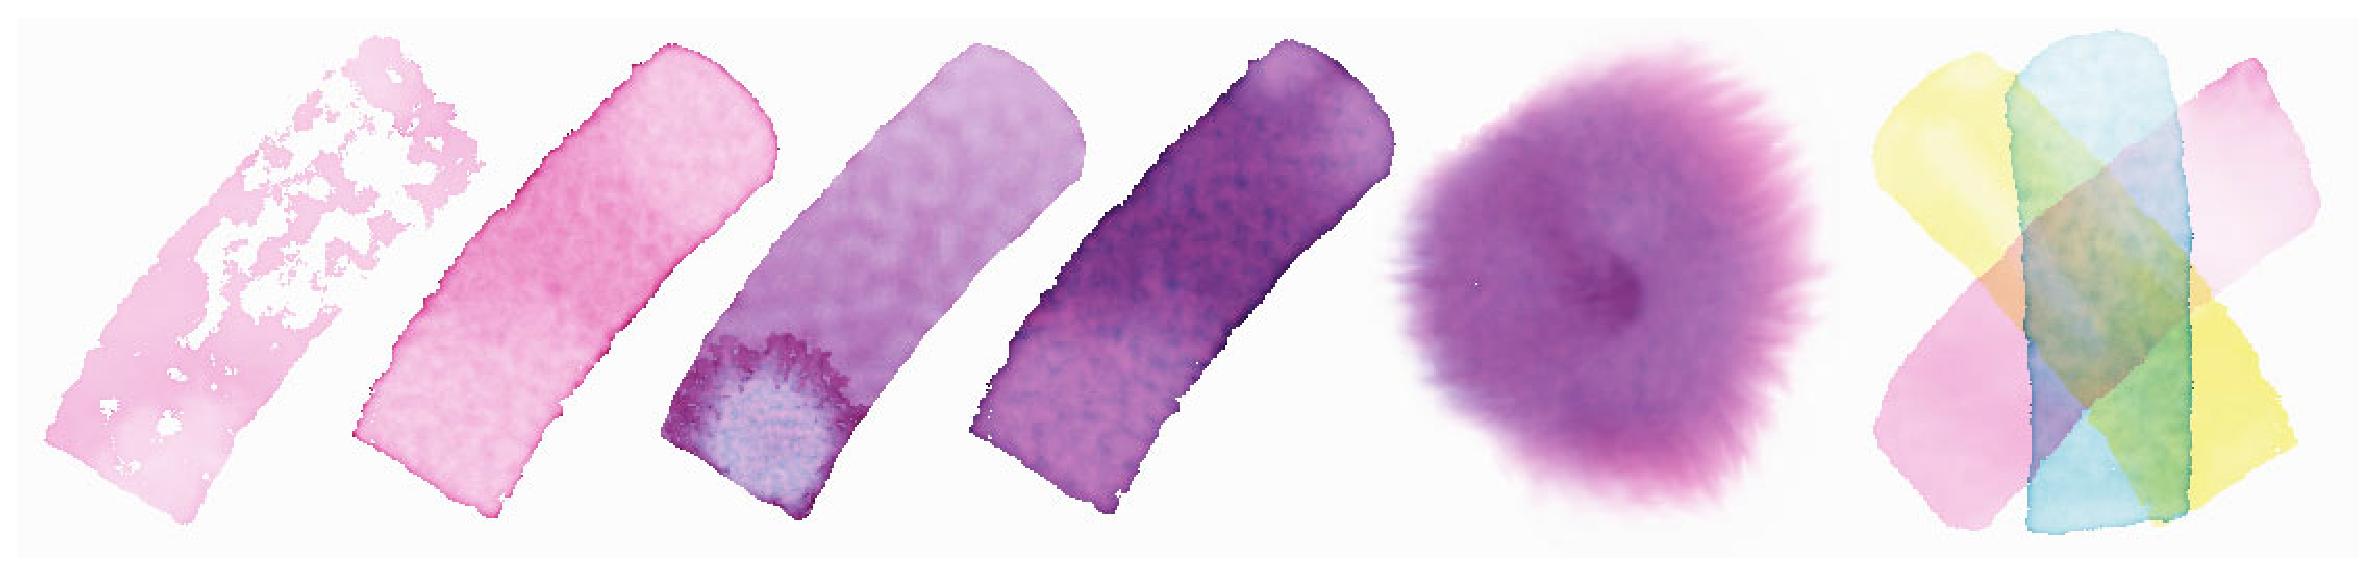
\includegraphics[width=1.00\textwidth]{../images/Curtis1997-simulated-watercolor-effects.eps}
  \caption{Simulierte Wasserfarbeneffekte. Quelle: \cite{Curtis1997}.}
  \label{fig:effects-simulated}
\end{figure}

\subsubsection{Papier}
Die Struktur des Papiers beeinflusst in der Realität maßgeblich die 
Flüssigkeitsbewegungen, den \textsl{granulation}- sowie den 
\textsl{backrun}-Effekt. Bei der Simulation gelangt ein vereinfachtes 
Papiermodell zum Einsatz: Die Textur des Papiers wird als ein Höhen- und 
Flüssigkeitskapazitätsfeld abgebildet. Das Höhenfeld $h$ wird zufällig bestimmt 
und auf das Intervall $[0,1]$ skaliert. Zur späteren Berechnung der 
Flüssigkeitsgeschwindigkeiten $u$ und $v$ wird die Steigung des Höhenfeldes 
berechnet. Die Flüssigkeitskapazität $c$ ergibt sich aus dem Höhenfeld:
\[
c = h (c_{max} - c_{min}) + c_{min}
\]

\subsubsection{3-Schichten-Modell}
Jeder Wasserfarben-Layer wird mittels des in Abbildung 
\ref{fig:3-schichten-modell} gezeigten Schichten-Modells simuliert.

\begin{figure}
  \centering
  \subfloat[shallow-water layer]{
    \label{fig:3-schichten-modell-shallow}
    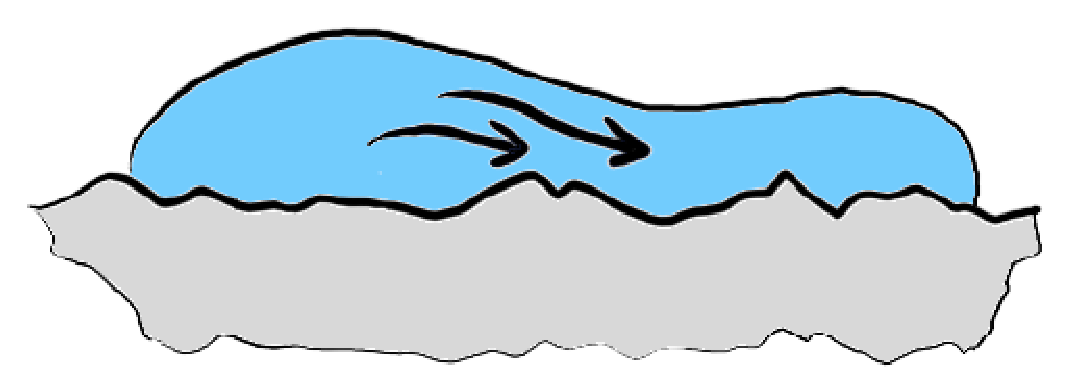
\includegraphics[width=0.30\textwidth]{../images/Curtis1997-layer-shallow-water}
  }
  \par
  \subfloat[pigment-deposition layer]{
    \label{fig:3-schichten-modell-pigment}
    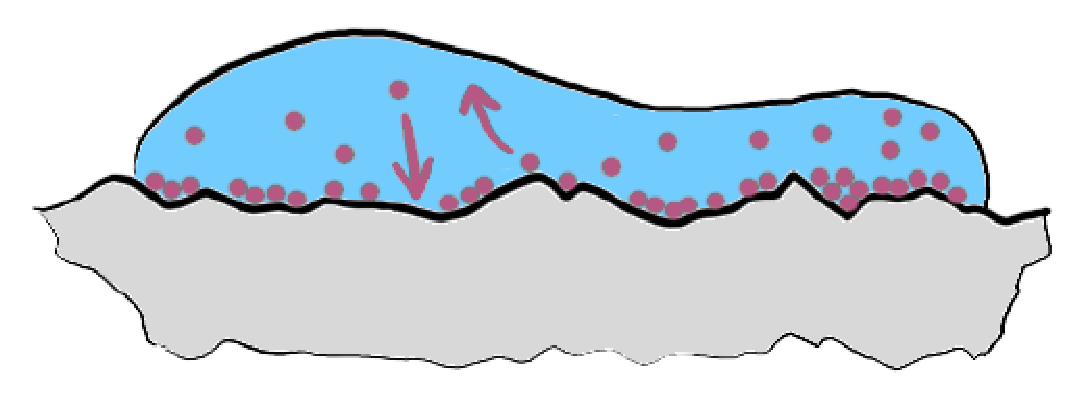
\includegraphics[width=0.30\textwidth]{../images/Curtis1997-layer-pigment-deposition}
  }
  \par
  \subfloat[capillary layer]{
    \label{fig:3-schichten-modell-capillary}
    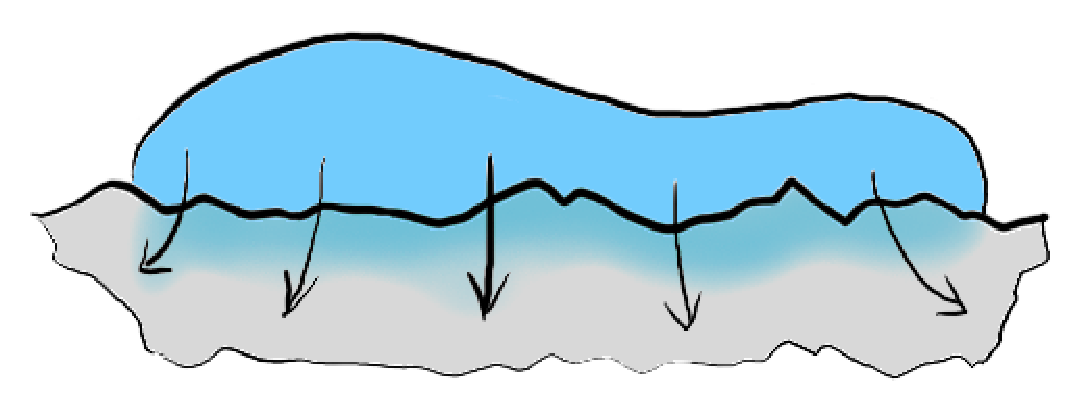
\includegraphics[width=0.30\textwidth]{../images/Curtis1997-layer-capillary}
  }
  \caption{3-Schichten-Modell für die Flüssigkeitssimulation. Quelle: \cite{Curtis1997}.}
  \label{fig:3-schichten-modell}
\end{figure}

Die einzelnen Schichten haben dabei von oben nach unten die folgenden Bedeutungen
und Aufgaben:

\begin{itemize}
  \item Innerhalb des \textsl{shallow-water layer} (dt.\ Flachwasserschicht, 
  Abb.\ \ref{fig:3-schichten-modell-shallow}) können das Wasser und 
  Farbpigmente über die Papieroberfläche transportiert werden.
  \item Auf dem \textsl{pigment-deposition layer} (dt.\ 
  Pigmentablagerungsschicht, Abb.\ \ref{fig:3-schichten-modell-pigment}) 
  können Pigmente abgelagert, bzw.\ von hier auch erneut weiter transportiert 
  werden.
  \item Im \textsl{capillary layer} (dt.\ Kapillarschicht, Abb.\ 
  \ref{fig:3-schichten-modell-capillary}) diffundiert das in das Papier 
  absorbierte Wasser und kann sich somit ausbreiten.
\end{itemize}

\subsubsection{Hauptschleife}
In Listing \ref{lst:mainloop} ist die Hauptschleife der Simulation in 
Pseudocode aufgeführt. Folgende Werte werden der Simulation als Anfangsdaten
übergeben: 

\begin{itemize}
  \item $M$, die sog.\ \textsl{wet-area mask}, die markiert, an welchen Stellen
  das Papier nass ($1$) bzw.\ trocken ist ($0$).
  \item $u$ und $v$, die Geschwindigkeit des Wassers in $x$- bzw.\ $y$-Richtung.
  \item $p$, der Wasserdruck.
  \item $g^k$, die Pigmentkonzentration.
  \item $d^k$, die abgesetzten Pigmente im \textsl{pigment-deposition layer}.
  \item $s$, die Wassersättigung des Papiers.
\end{itemize}

\begin{lstlisting}[caption={Simulationshauptschleife}, label={lst:mainloop}, %
emph={MoveWater, MovePigment, TransferPigment, SimulateCapillaryFlow}, %
emphstyle=]
function MainLoop($M$, $u$, $v$, $p$, $g^1$, ..., $g^n$, $d^1$, ..., $d^n$, $s$):
	for each time step do: (*\label{line:time-step}*)
		MoveWater($M,$ $u$, $v$, $p$)
		MovePigment($M$, $u$, $v$, $g^1$, ..., $g^n$)
		TransferPigment($g^1$, ..., $g^n$, $d^1$, ..., $d^n$)
		SimulateCapillaryFlow($M$, $s$)
	end for
end function
\end{lstlisting}

Wie das Listing zeigt, iteriert die Simulation über eine definierte Anzahl von 
Zeitschritten (Zeile \ref{line:time-step}), führt Wasser- und Pigmentbewegungen 
aus, transferiert Pigmente zwischen den verschiedenen Schichten, haftet diese 
an das Papier an und lässt Wasser durch den \textsl{capillary layer} 
diffundieren.

\subsubsection{Simulationsschritte}
\paragraph{Wasserbewegung} 
Die Bewegungen des Wassers werden im \textsl{shallow-water layer} durchgeführt. 
Einige der Bedingungen für das Verhalten des Wassers lauten dabei:

\begin{enumerate}
  \item Der Wasserfluss muss begrenzt werden durch die \textsl{wet-area mask}.
  \item Wasserüberschuss in einer Region sollte ein Abfließen des Überschusses in
  benachbarte Regionen verursachen.
  \item Lokale Änderungen (z.\,B.\ das Hinzufügen von Wasser an einer Stelle) 
  sollten Auswirkungen auf die komplette Simulation haben.
\end{enumerate}

Listing \ref{lst:watermovement} zeigt die grobe Vorgehensweise bei der 
Simulation der Wasserbewegungen.

\begin{lstlisting}[caption={Wasserbewegung}, label={lst:watermovement}, %
emph={MoveWater, UpdateVelocities, RelaxDivergence, FlowOutward}, %
emphstyle=]
function MoveWater(M, u, v, p):
	UpdateVelocities(M, u, v, p)
	RelaxDivergence(M, u, v, p)
	FlowOutward(M, p)
end function
\end{lstlisting}

Auf die einzelnen Untermethoden soll hier nicht weiter eingegangen, sondern 
deren Funktion nur kurz umrissen werden. \textsl{UpdateVelocities()} ist für
die Aktualisierung der Wassergeschwindigkeiten $u$ und $v$ zuständig.
\textsl{RelaxDivergence()} dient dazu, die Abweichungen des
Geschwindigkeitsfelds zu entspannen. Mittels \textsl{FlowOutward()} wird
schließlich der \textsl{edge darkening}-Effekt simuliert, indem in jedem 
Schritt eine proportional zur Entfernung zum Rand steigende Wassermenge aus den 
Zellen entfernt wird.

\paragraph{Pigmentbewegung}
Pigmente bewegen sich innerhalb der Flachwasserschicht gemäß dem zuvor
berechneten Geschwindigkeitsfeld $u, v$ für das Wasser. Pigmente werden
entsprechend der Flüssigkeitsabflussrate aus einer Zelle in die Nachbarzellen
bewegt. Nachfolgend ist der Pseudocode für die Simulation der Pigmentbewegungen
angegeben. 

\begin{lstlisting}[caption={Pigmentbewegung}, label={lst:pigmentmovement}, %
morekeywords={forall}]
function MovePigment(M, u, v, $g^1$, ..., $g^n$):
	$\Delta t$ = $1/\lceil \max_{i,j}\{|u|, |v|\} \rceil$

	for each pigment k do
		for t = 0 to 1 by $\Delta t$ do
			$g'$ = $g$ = $g^k$

			forall cells ($i$, $j$) do
				$g'_{i+1,j}$ = $g'_{i+1,j}$ + $\max(0, u_{i+0.5,j} g_{i,j})$
				$g'_{i-1,j}$ = $g'_{i-1,j}$ + $\max(0, -u_{i-0.5,j} g_{i,j})$
				$g'_{i,j+1}$ = $g'_{i,j+1}$ + $\max(0, v_{i,j+0.5} g_{i,j})$
				$g'_{i,j-1}$ = $g'_{i,j-1}$ + $\max(0, -v_{i,j-0.5} g_{i,j})$
				$g'_{i,j}$ = $g'_{i,j}$ - $\max(0, u_{i+0.5,j} g_{i,j})$ + $\max(0, -u_{i-0.5,j} g_{i,j})$ + $\max(0, v_{i,j+0.5} g_{i,j})$ + $\max(0, -v_{i,j-0.5} g_{i,j})$
			end for
			$g^k$ = $g'$
		end for
	end for
end function
\end{lstlisting}

\paragraph{Pigmentabsorption und -desorption}
In jedem Simulationsschritt werden Pigmente zu einem gewissen Grad von der 
Pigmentablagerungsschicht absorbiert und auch wieder zurück in die Flüssigkeit 
resorbiert. Mittels der Parameter \textsl{density} (Dichte) und 
\textsl{staining power} (Verschmutzungsfähigkeit) lässt sich festlegen, in 
welchem Maße jedes Pigment ab- bzw.\ resorbiert wird. Weiterhin bestimmt der 
Parameter \textsl{granulation} (Körnung), wie die Papierhöhe $h$ die Ab- und 
Resorption beeinflusst.

Für den Pseudocode dieses Simulationsschritts sei auf den entsprechenden 
Abschnitt der Arbeit von \cite{Curtis1997} verwiesen.

\paragraph{Backrun-Effekt}
Die sog.\ \textsl{Backruns} entstehen, wenn eine Wasserlache sich langsam über
eine trocknende, aber noch feuchte Region ausbreitet. In feuchten Regionen
verteilt sich Flüssigkeit nicht mehr in der Flachwasserschicht, sondern über die
Kapillareffekte in der entsprechenden Kapillarschicht.
Zur Simulation dieses Effekts wird Wasser aus der Flachwasserschicht absorbiert
und diffundiert durch die Kapillarschicht. Jede Zelle überträgt dabei solange
Wasser an die Nachbarzellen, bis diese bis zur Kapazität $c$ gesättigt sind.
Liegt diese Sättigung nun über einem Schwellwert, so wird die \textsl{wet-area
mask} entsprechend erweitert - auf diese Weise kann sich eine Wasserlache durch
die Kapillarvorgänge ausbreiten.

Wie zuvor verweisen wir für den Pseudocode auf die Arbeit von \cite{Curtis1997}.

\subsubsection{Rendering der Wasserfarbenlayer}
Nach Berechnung der einzelnen Wasserfarbenlayer werden diese mithilfe des 
Kubelka-Munk-Farbmodells (KM-Farbmodell) zusammengefügt. Dieses Farbmodell 
erlaubt eine realistischere, aber dementsprechend aufwändigere Darstellung von 
Farbeffekten als z.\,B.\ das RGB-Farbmodell. Es werden dabei für jeden 
Farbkanal des RGB-Farbraums zwei Koeffizienten berechnet:

\begin{enumerate}
  \item Der Absorptionskoeffizient $K$ bestimmt den Anteil der absorbierten 
  Energie.
  \item Der Streuungskoeffzient $S$ bestimmt den Anteil der zurückgestreuten 
  Energie.
\end{enumerate}

Im Gegensatz zur typischen Anwendung der KM-Theorie werden diese Koeffizienten 
nicht experimentell bestimmt, sondern lassen sich vom Benutzer interaktiv 
festlegen. Auf diese Weise lassen sich eine große Anzahl realistisch wirkender 
Farben erzeugen, wie Abbildung \ref{fig:pigments} beispielhaft zeigt.

\begin{figure}
  \centering
  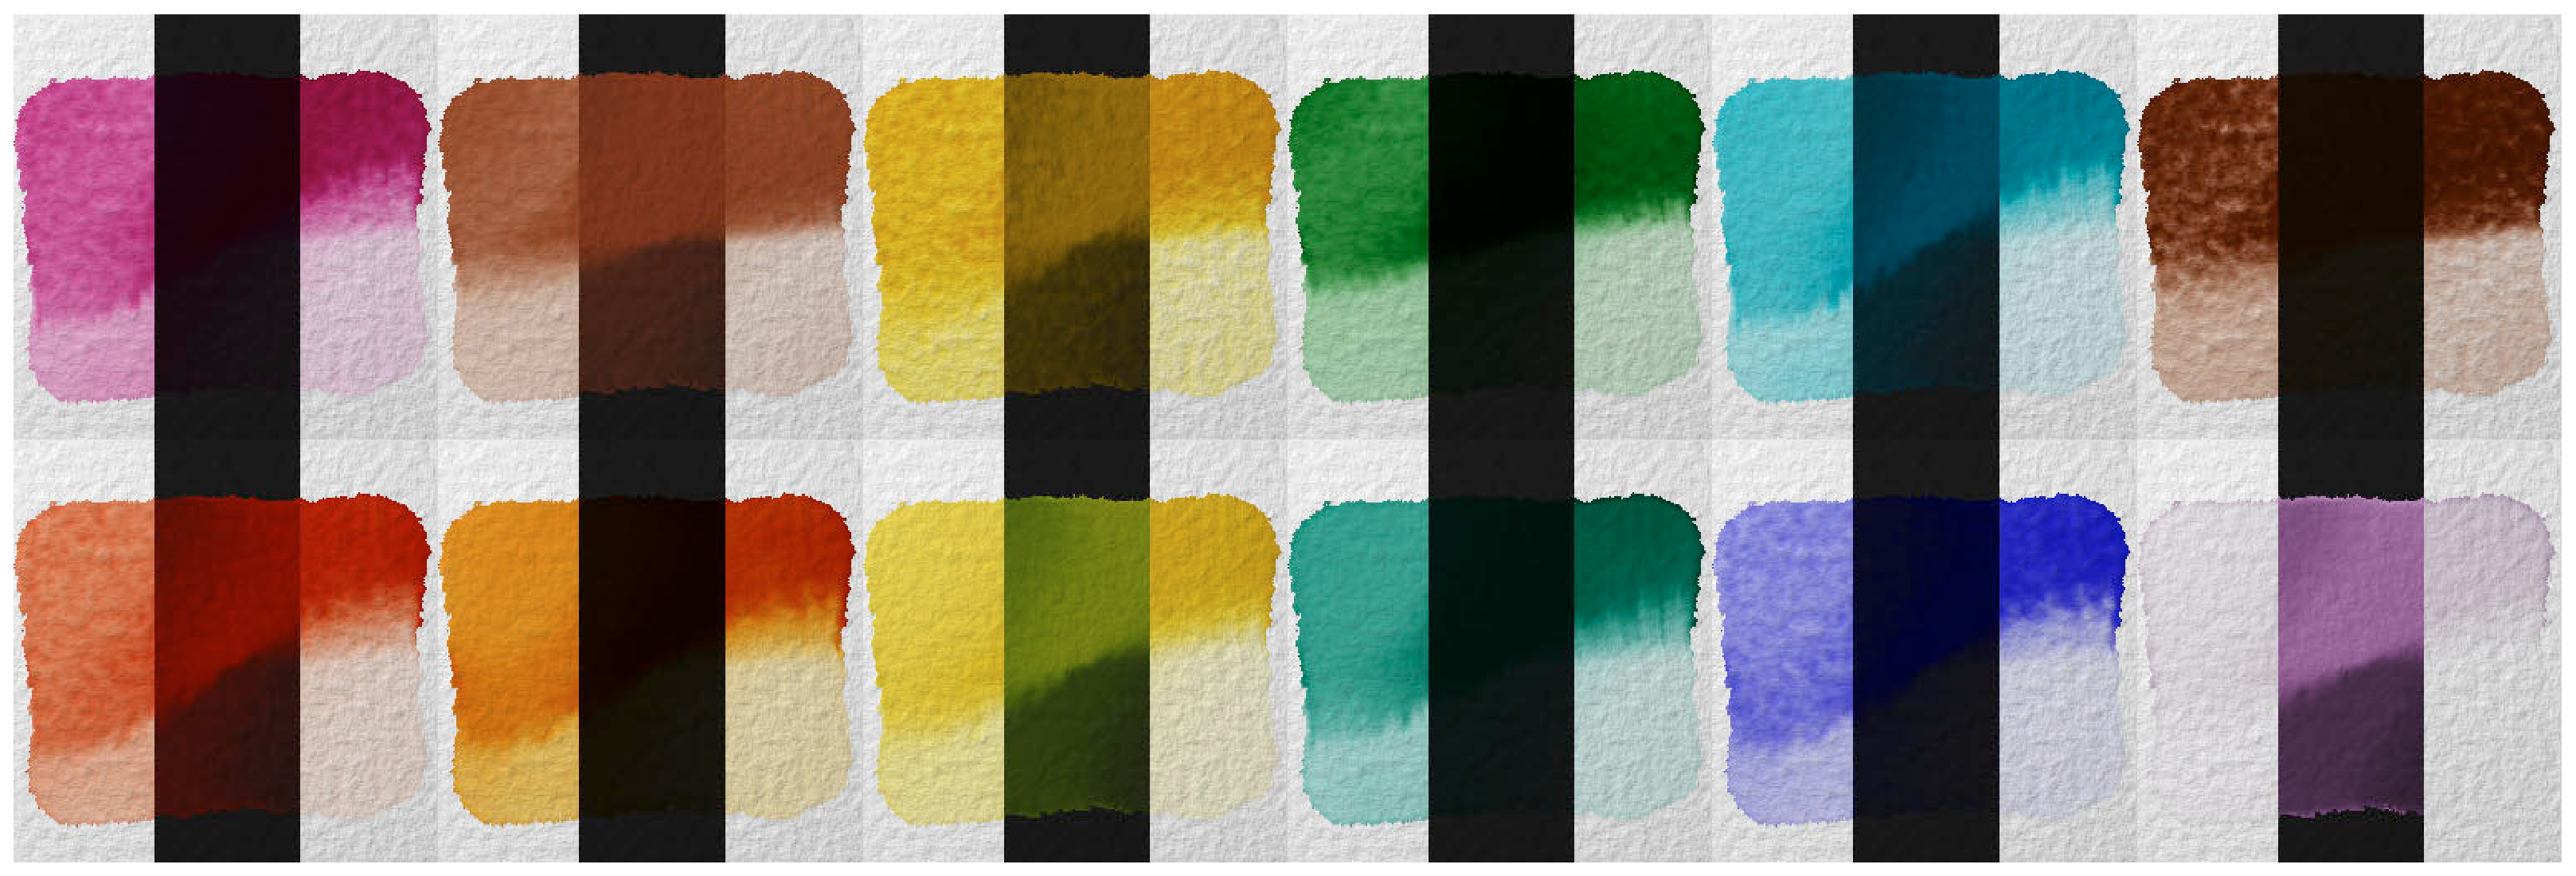
\includegraphics[width=1.00\textwidth]{../images/Curtis1997-pigments}
  \caption{Verschiedene synthetisch erzeugte Pigmente. Quelle: \cite{Curtis1997}.}
  \label{fig:pigments}
\end{figure}

\paragraph{Komposition der Layer}
Nach Ermittlung der Koeffizienten $K$ und $S$ für einen Layer der Dicke $x$ 
kann nun mithilfe des KM-Modells die Reflektion $R$ und der 
Durchlässigkeitsgrad $T$ bestimmt werden:

\begin{eqnarray*}
R &=& \sinh b S x/c \\
T &=& b/c, \qquad c = a \sinh b S x + b \cosh b S x \\
\end{eqnarray*}

Der Wert $x$ errechnet sich aus der Summe der Pigmentkonzentration $g^k$ in der 
Flachwasserschicht und der Konzentration der abgelagerten Pigmente $d^k$ in der 
Pigmentablagerungsschicht. Weiterhin können nun die Werte $R$ und $T$ für zwei 
angrenzende Layer errechnet werden:

\begin{eqnarray*}
  R &=& R_1 + \frac{T^2_1 R_2}{1 - R_1 R_2} \\
  T &=& \frac{T^1 T_2}{1 - R_1 R_2}
\end{eqnarray*}

Diese Berechnung wird für jeden zusätzlichen Layer wiederholt und schließlich
wird die Gesamtreflektion $R$ für die Darstellung des jeweiligen Pixels benutzt.

\subsection{Anwendungen}
Mithilfe des vorgestellten Simulationsverfahrens lassen sich eine Reihe von
Anwendungen realisieren.
Da ist zunächst das \textbf{interaktive Malen} zu erwähnen. Dem Anwender wird
ermöglicht, den "`Startzustand"' der Simulation interaktiv zu malen. Dabei
erstellt er beliebig viele Wasserfarbenlayer, die jeweils Unterlayer für die
Pigmente, das Wasser und die \textsl{wet-area mask} besitzen. Allen Layern
gemein ist ein Referenzbild sowie eine Papiertextur. Außerdem lassen sich
jeweils die physikalischen Eigenschaften der einzelnen Layer sowie die Anzahl
der Simulationsschritte festlegen.
Da die Simulation wie gezeigt doch recht komplex ist, kann diese nicht in
Echtzeit ablaufen. In Kapitel \ref{sec:echtzeit-wasserfarben} stellen wir einen
weiteren Ansatz vor, der Wasserfarbenanimationen von 3D-Szenen in Echtzeit 
erlaubt.

Eine weitere Anwendung ist die sog.\ \textbf{Watercolorization}, bei der ein 
bestehendes Farbbild in eine Wasserfarben-Illustration transformiert wird. Dazu 
wird zunächst eine Farbtrennung durchgeführt, bei der ermittelt wird, in 
welchem Layer welche Pigmentfarbe zu platzieren ist. Anschließend werden beim 
Malen jedes Layers Wasser- oder Pigmentpinselstriche hinzugefügt, um dem 
Ausgangsbild möglichst nah zu kommen. Abbildung \ref{fig:watercolorization} 
zeigt beispielhaft das Ergebnis einer solcher automatischen Kolorierung. Als 
Erweiterung lässt sich dieses Verfahren auch auf 3D-Szenen anwenden.

\begin{figure}
  \centering \subfloat[Ausgangsbild]{
    \label{fig:watercolorization-input}
  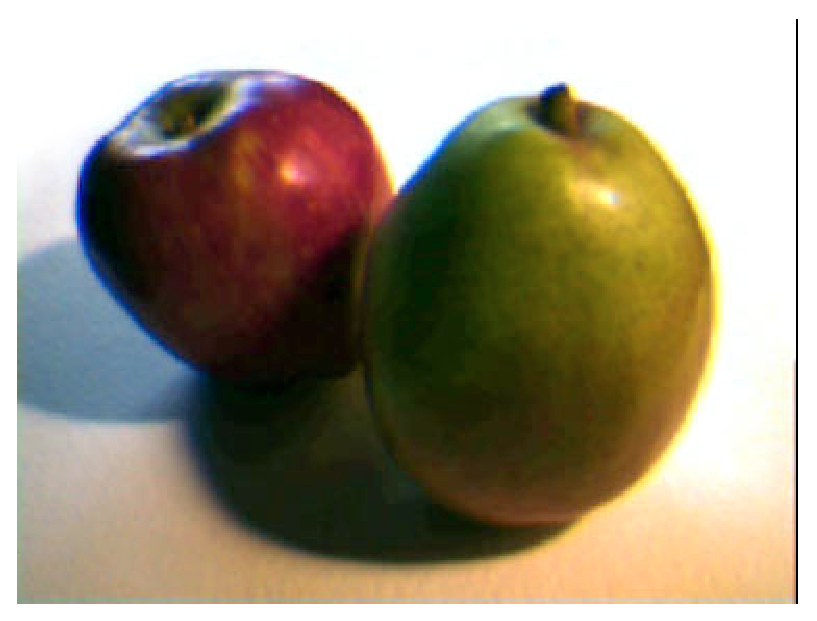
\includegraphics[width=0.40\textwidth]{../images/Curtis1997-watercolorization-input} 
  } \subfloat[Ergebnisbild mit 11 Layern]{
    \label{fig:watercolorization-output}
  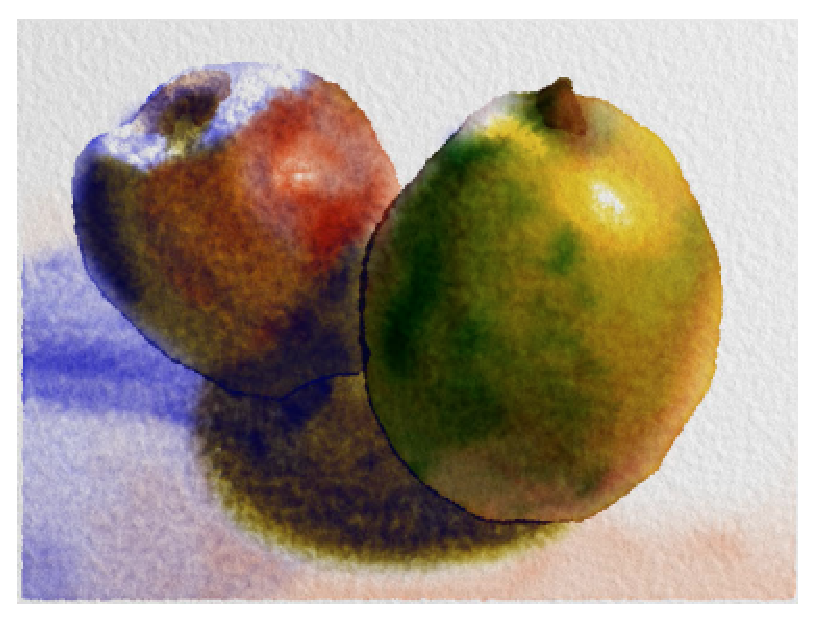
\includegraphics[width=0.40\textwidth]{../images/Curtis1997-watercolorization-output} 
  }
  \caption{Watercolorization, Anzahl der Simulationsschritte: 2750. Quelle: \cite{Curtis1997}.}
  \label{fig:watercolorization}
\end{figure}

\section{Echtzeit-Wasserfarben-Animationen}
\label{sec:echtzeit-wasserfarben}

\subsection{Einleitung}
Im Gegensatz zur zuvor beschriebenen physikalischen Simulation von Wasserfarben 
beschreibt die Arbeit von \cite{Luft2006} Verfahren, mit denen möglichst 
naturgetreue Animationen in Wasserfarbenoptik von 3D-Szenen in 
\textsl{Echtzeit} erstellt werden können. Wie bereits gesehen, erfordert die 
realistische Simulation einen hohen Aufwand, weshalb man sich hier für einen 
Mittelweg zwischen möglichst überzeugender Darstellung und hoher 
Geschwindigkeit der Animation entschieden hat. Es werden die wichtigsten 
Effekte der Wasserfarbenmalerei imitiert und außerdem Licht- und 
Schatteneffekte erzeugt.

\subsection{Abstraktion und Vereinfachung}
Der erste Schritt des Verfahrens beinhaltet die Erstellung einer Anzahl 
abstrakter Wasserfarbenlayern, die alle mehr oder weniger einen gleichförmigen 
Inhalt bzw.\ Farbe haben. In Abbildung \ref{fig:tree-original} sind dies 
beispielsweise die Blätter auf der einen und die Äste auf der anderen Seite. 
Die Ausgangs-3D-Szene wird anhand eindeutiger Identifikatoren segmentiert, das 
Ergebnis (s.\ Abbildung \ref{fig:tree-segmentation}) sind die sog.\ 
\textsl{intensity images} $\rho : \mathbf{N}^2 \to \mathbf{R}$, wobei $\rho(x, 
y) \in [0,1]$. Anschließend wird mithilfe eines Tiefpassfilters (Gauss-Filter) 
der gewünschte Abstraktionsgrad erzielt; es entstehen abstrakte weiche Formen. 
Außerdem erhält jeder Layer eine benutzerdefinierte Farbe $c_{rgb}$ sowie 
Transparenz $c_a$.

\begin{figure}
  \centering
  \subfloat[Photorealistisches Originalmodell]{
    \label{fig:tree-original}
    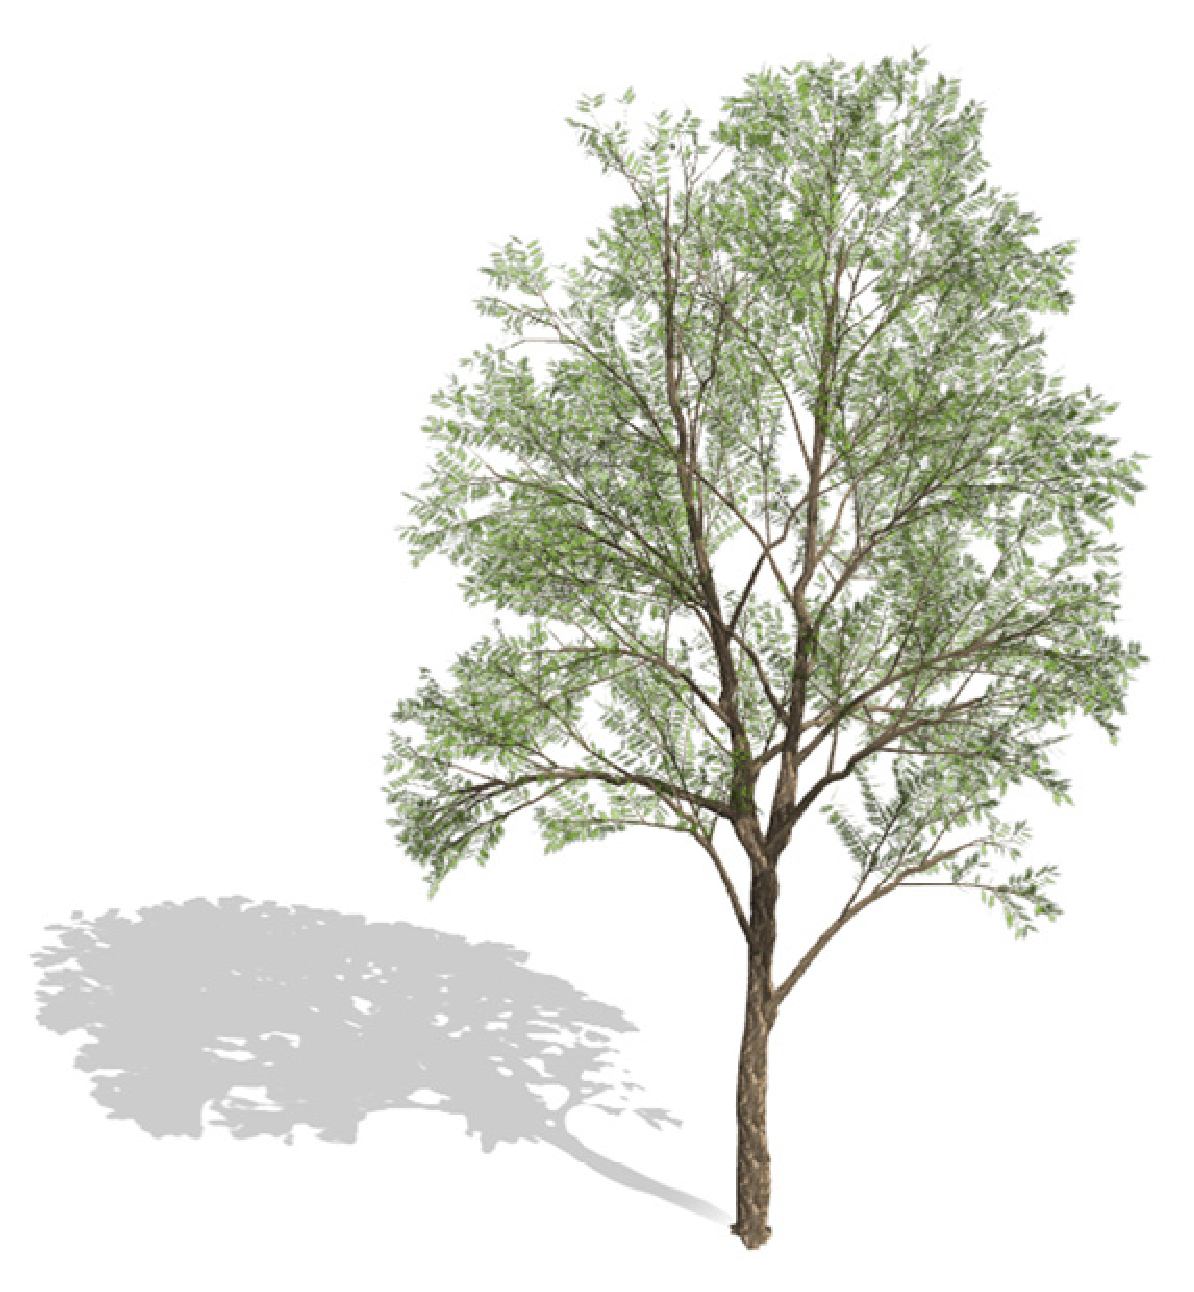
\includegraphics[height=6cm]{../images/Luft2006-tree-original}
  }
  \qquad
  \subfloat[Ergebnis nach der Segmentierung]{
    \label{fig:tree-segmentation}
    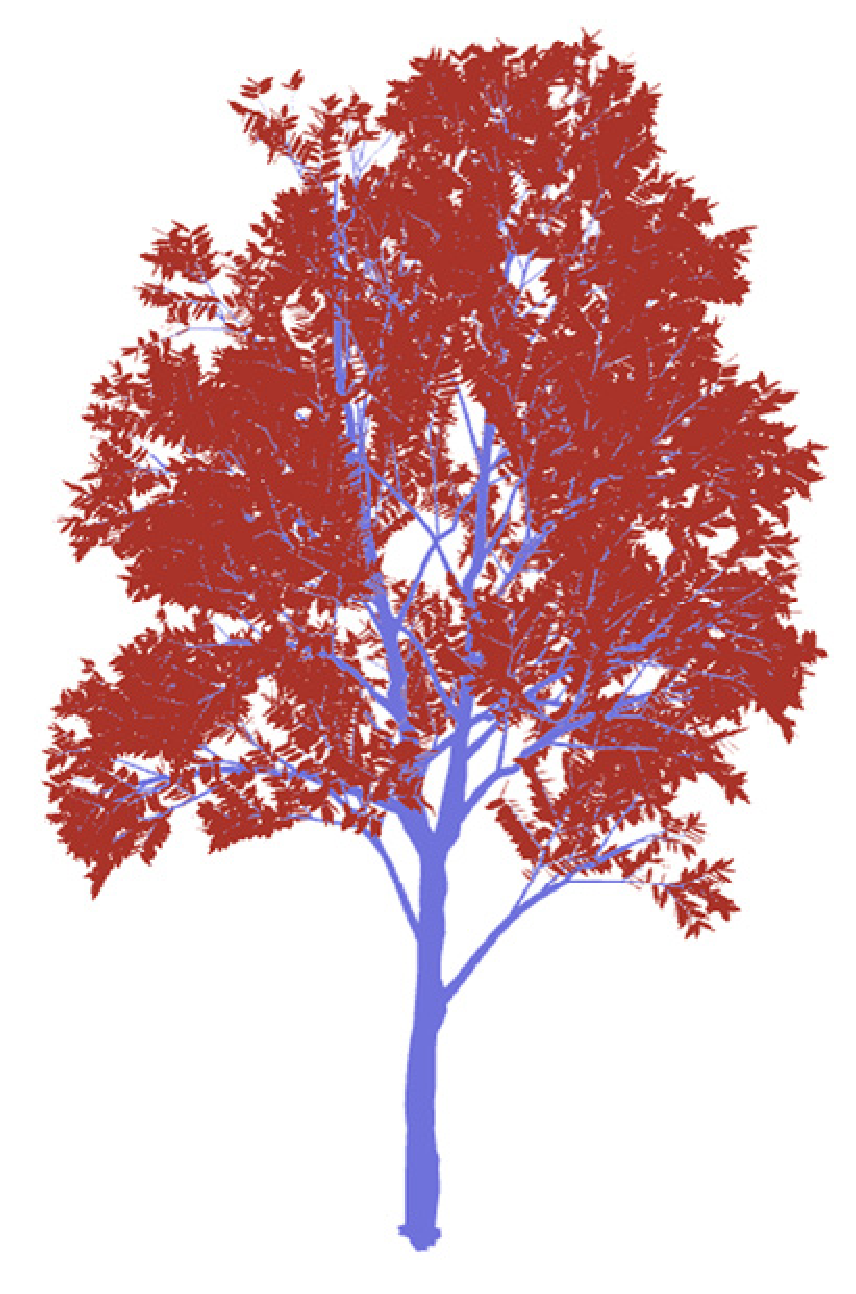
\includegraphics[height=6cm]{../images/Luft2006-tree-segmentation}
  }
  \caption{Abstraktion und Vereinfachung. Quelle: \cite{Luft2006}.}
  \label{fig:original-segmentation}
\end{figure}

\subsection{Formextraktion und Fließmuster}
Die Form eines Wasserfarbenlayers ergibt sich direkt aus den Intensitätswerten 
des entsprechenden \textsl{intensity image} $\rho(x, y)$. Zur Erzeugung einer 
hartkantigen Form des Wasserfarbenlayers wird eine \textsl{step}-Funktion 
angewandt und eine initiale Transparenz berechnet:

\[
\lambda_a(x,y) = c_a \cdot step(\kappa_\rho, \rho(x,y))
\]

Mittels des Parameters $\kappa_\rho$ lässt sich die Ausdehnung des 
Wasserfarbenlayers beeinflussen. Zur Erzeugung der Fließmuster wird die 
\textsl{step}-Funktion durch eine andere Variante ersetzt, bei welcher über 
einen zusätzlichen Parameter die Weichheit der Kanten bestimmt wird - auf diese 
Weise lassen sich das \textsl{wet-on-dry}- und \textsl{wet-on-wet}-painting 
imitieren.

\subsection{Edge darkening}
Dieser bereits beschriebene Effekt wird durch Anwendung des Gauss-Filters
ermöglicht, welcher einen weichen Intensitätsübergang an den Kanten der Layers
erzeugt. Um den Effekt naturgetreu zu imitieren, muss zusätzlich der Rand
verdunkelt dargestellt werden. Dazu wird der Alpha-Kanal $\lambda_a(x,y)$ mittels
der Intensitätswerte angepasst:

\[
\lambda_a(x,y) = \lambda_a(x,y) \cdot (1 + \kappa_\omega \cdot (1 - \rho(x,y)))
\]

Über den Parameter $\kappa_\omega$ kann der Anwender also die Stärke der
Kantenabdunklung festlegen, ein Beispiel nach Durchführung zeigt Abbildung
\ref{fig:tree-edge-darkening}.

\begin{figure}
  \centering
  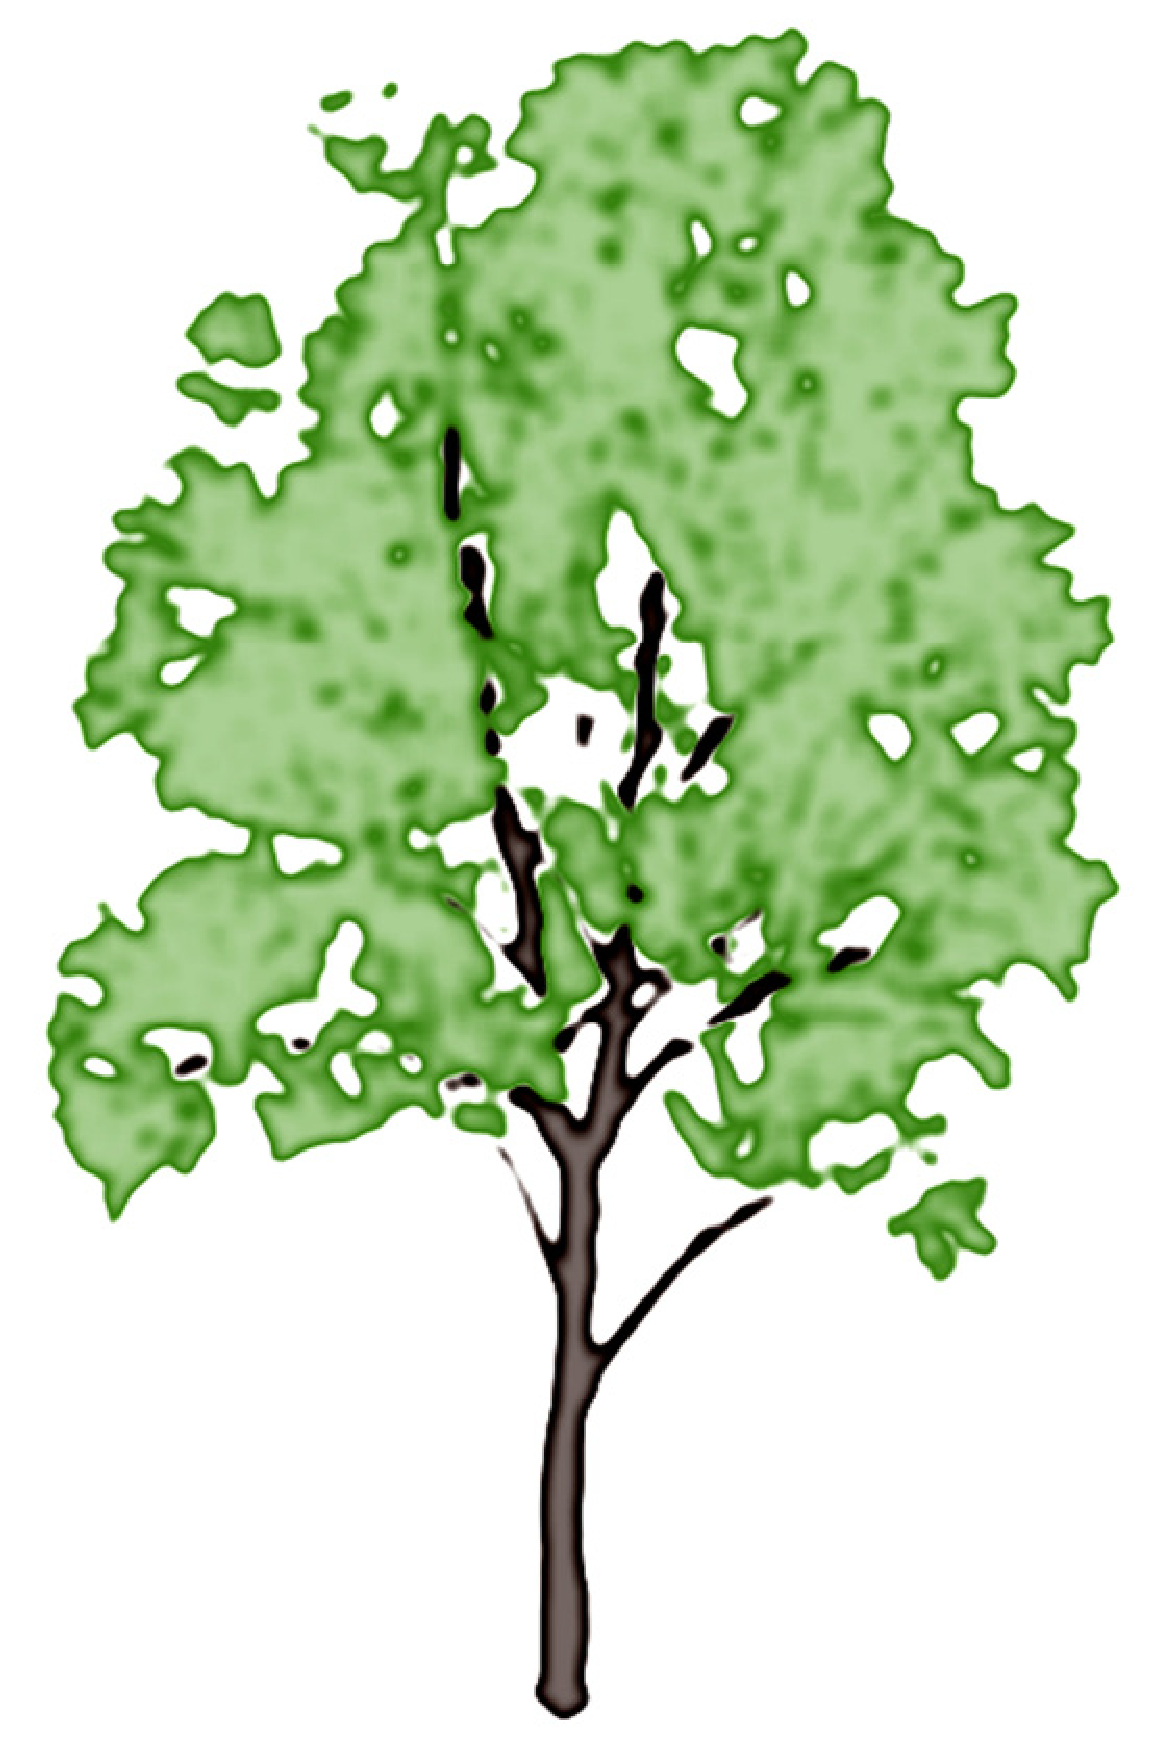
\includegraphics[height=6cm]{../images/Luft2006-tree-edge-darkening}
  \caption{Edge darkening mit $\kappa_\omega = 0.8$. Quelle: \cite{Luft2006}.}
  \label{fig:tree-edge-darkening}
\end{figure}

\subsection{Komposition der Wasserfarben-Layern}
Nach der Erstellung der einzelnen Layer werden evtl.\ zusätzliche Schichten für
Farb- und Schatteneffekte erstellt und aus allen Layern schließlich das
Ergebnisbild zusammengesetzt.

\subsubsection{Licht und Schatten}
Die bereits beschriebene Methode zur Segmentierung der 3D-Szenen ignoriert
all diejenigen Oberflächendetails, die auf Licht und Schatten zurückzuführen
sind. Daher werden die im Modell evtl.\ verfügbaren Beleuchtungsinformationen
zur nachträglichen Anpassung der einzelnen Layer oder Erzeugung neuer verwendet.

Für die Erzeugung der \textbf{Beleuchtungseffekte} wird das 
Phong-Beleuchtungsmodell \cite{Phong1975} benutzt. In diesem Modell wird die 
Reflextion von Licht als Kombination aus ambienter, ideal diffuser und ideal 
spiegelnder Reflexion betrachtet. In diesem Falle wird der ambiente Term als 
konstant und bereits durch die initiale Farbe der Layer gegeben angenommen. Die 
verbleibenden zwei Komponenten werden aus Optimierungsgründen zunächst auf das 
Intervall $[0,1]$ normiert und anschließend auf zwei getrennte \textsl{lighting 
maps} gerendert:

\[
L_d, L_s : \mathbb{N}^2 \to \mathbb{R}
\]

Mithilfe dieser zusätzlichen Layer werden dann alle Wasserfarbenlayer
manipuliert:

\begin{itemize}
  \item Der spiegelnde Term entspricht einer Reflexion von Licht und erzeugt
  somit einen hervorgehobenen Bereich. Objekte, welche aus einem spiegelnden
  Material bestehen, müssen also im \textsl{intensity image} mithilfe der
  entsprechenden \textsl{lighting map} vor Erstellung des Wasserfarbenlayers 
  ausmaskiert werden: 
  \[
  \rho(x,y) = \rho(x,y) \cdot (1- step(\kappa_s, L_s(x,y)))
  \]
  \item Der diffuse Term wird analog dazu benutzt, um neue Layer zu erstellen,
  die dann als Maske für die \textsl{intensity images} benutzt werden. Weiterhin
  werden über diesen Term alle existierenden Wasserfarbenlayer in ihrer Farbe
  angepasst, um das entsprechende diffuse Umgebungslicht zu simulieren.
\end{itemize}

Um zusätzlich \textbf{Schatteneffekte} in die Szene zu integrieren, wird ein
zusätzlicher Layer erstellt, welcher nur die schattierten Regionen beinhaltet.
Zur Berechnung dieses Layers wird ein Standard-Algorithmus zur Berechnung von
Schatten verwendet. Die zuvor beschriebenen Effekte werden auf diesen
zusätzlichen Layer ebenfalls angewandt, inklusive des diffusen Umgebungslichts.

\subsubsection{Komposition}
Im Gegensatz zum Ansatz von \cite{Curtis1997} wird hier zur abschließenden 
Komposition (s.\ Abbildung \ref{fig:tree-result}) der einzelnen Layer nicht das 
Kubelka-Munk-Modell eingesetzt, sondern die Standard-Blending-Funktionen für 
transparente Objekte (Alpha-Blending). Die endgültige Farbe $C_{rgb}$ eines 
Pixels bestimmt sich mithilfe der Farbe $C_{rgb}$ und Transparenz $C_a$ des 
aktuellen Layers sowie der Hintergrundfarbe $B_{rgb}$:

\[
R_{rgb} = C_a \cdot C_{rgb} + (1 - C_a) \cdot B_{rgb}
\]

\begin{figure}
  \centering
  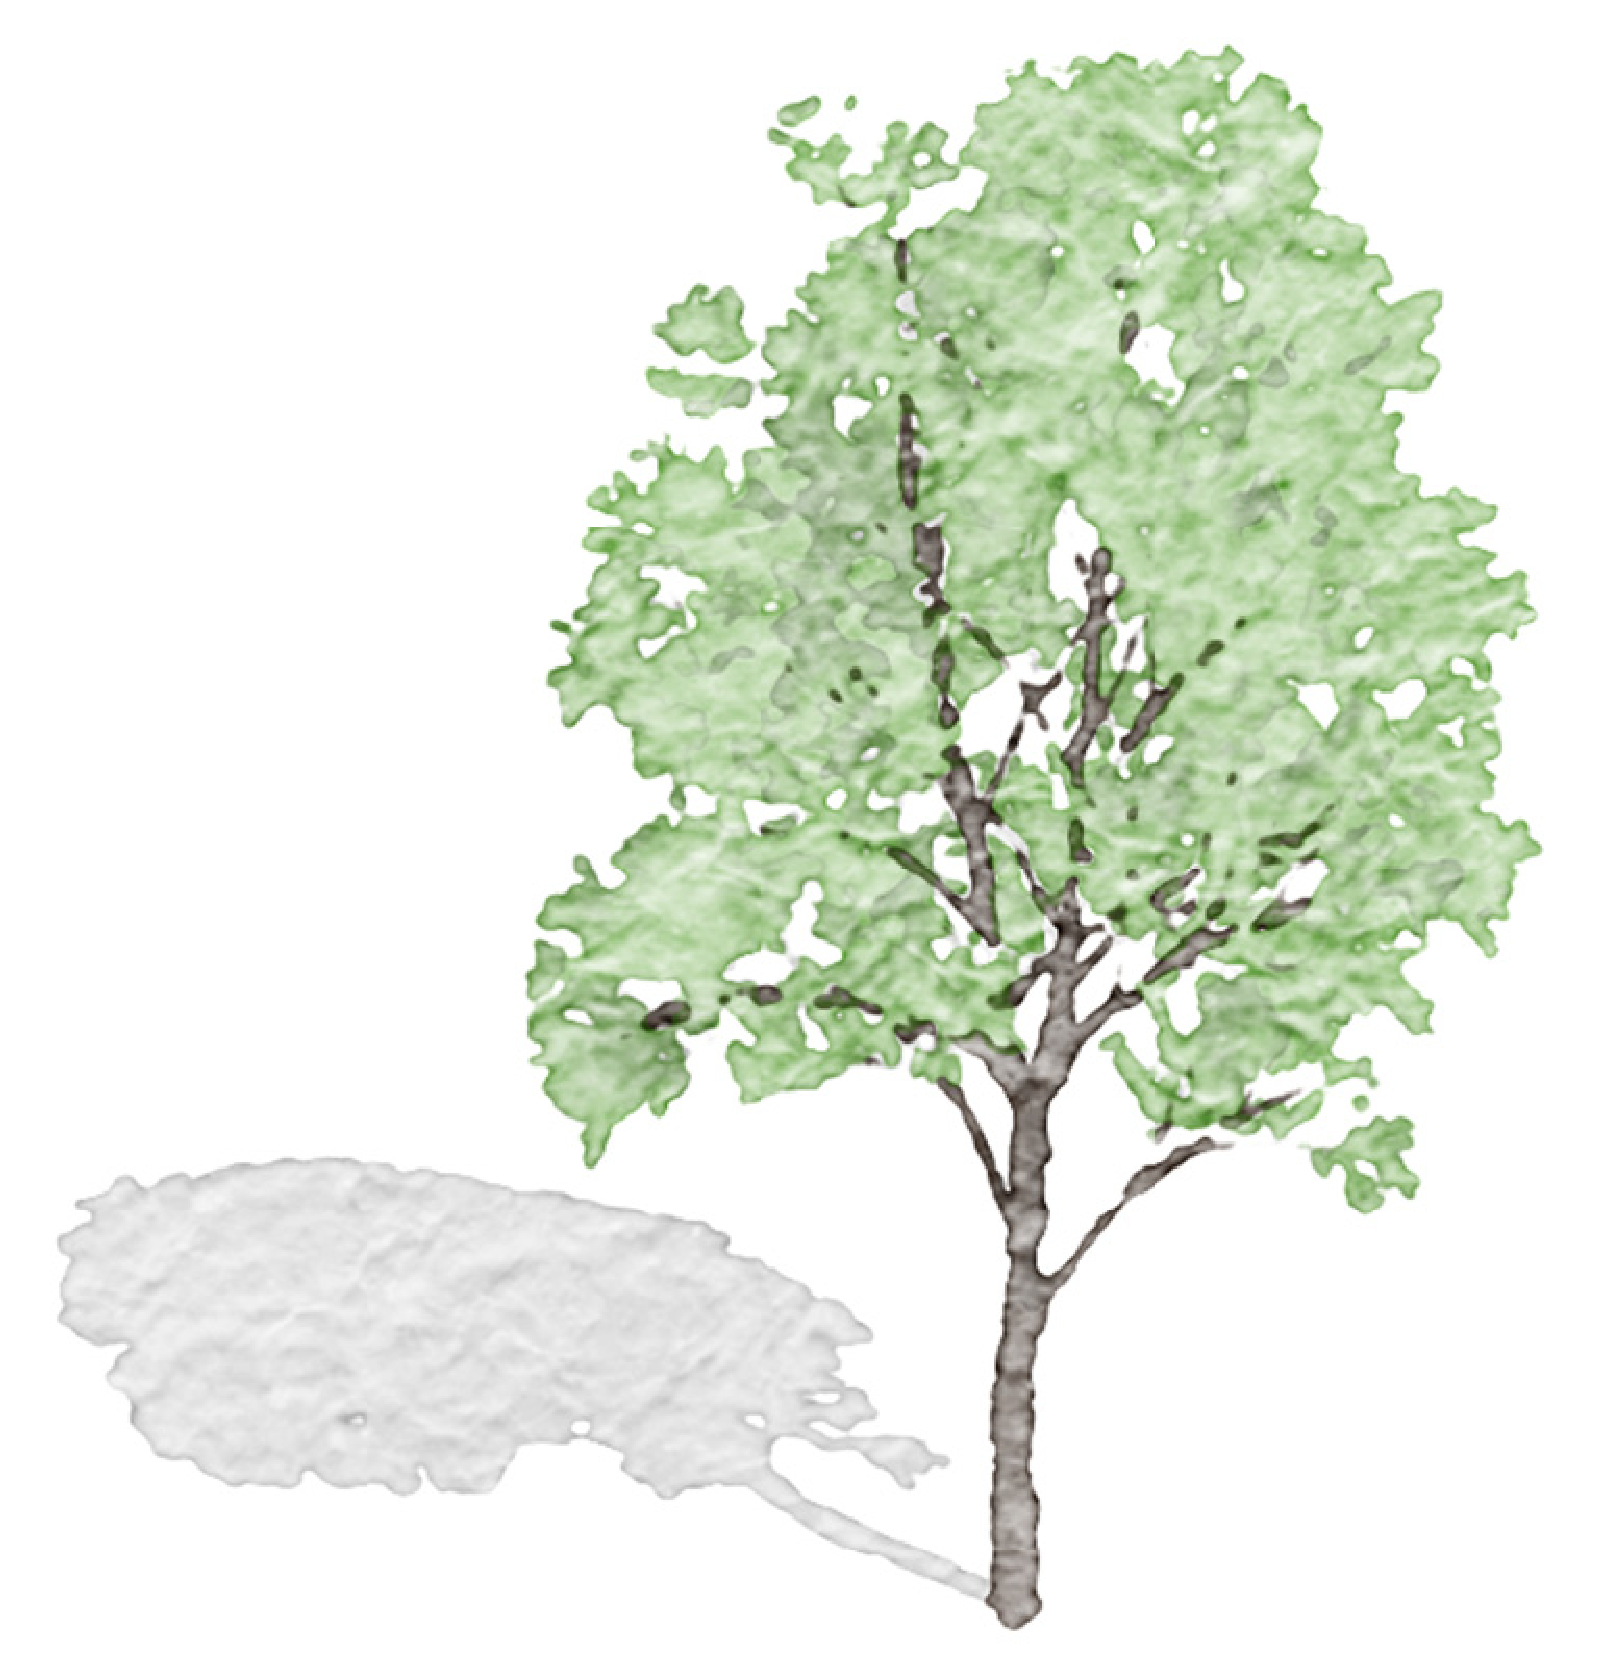
\includegraphics[height=6cm]{../images/Luft2006-tree-result}
  \caption{Endergebnis mit Schattenwurf. Quelle: \cite{Luft2006}.}
  \label{fig:tree-result}
\end{figure}

\subsection{Ergebnisse}
Abschließend stellen wir hier einige weiter Beispielbilder der Echtzeitanimation
vor. Alle Bilder wurden dabei mit einer Auflösung von 720 x 720 Pixel gerendert.

\begin{figure}
  \centering
  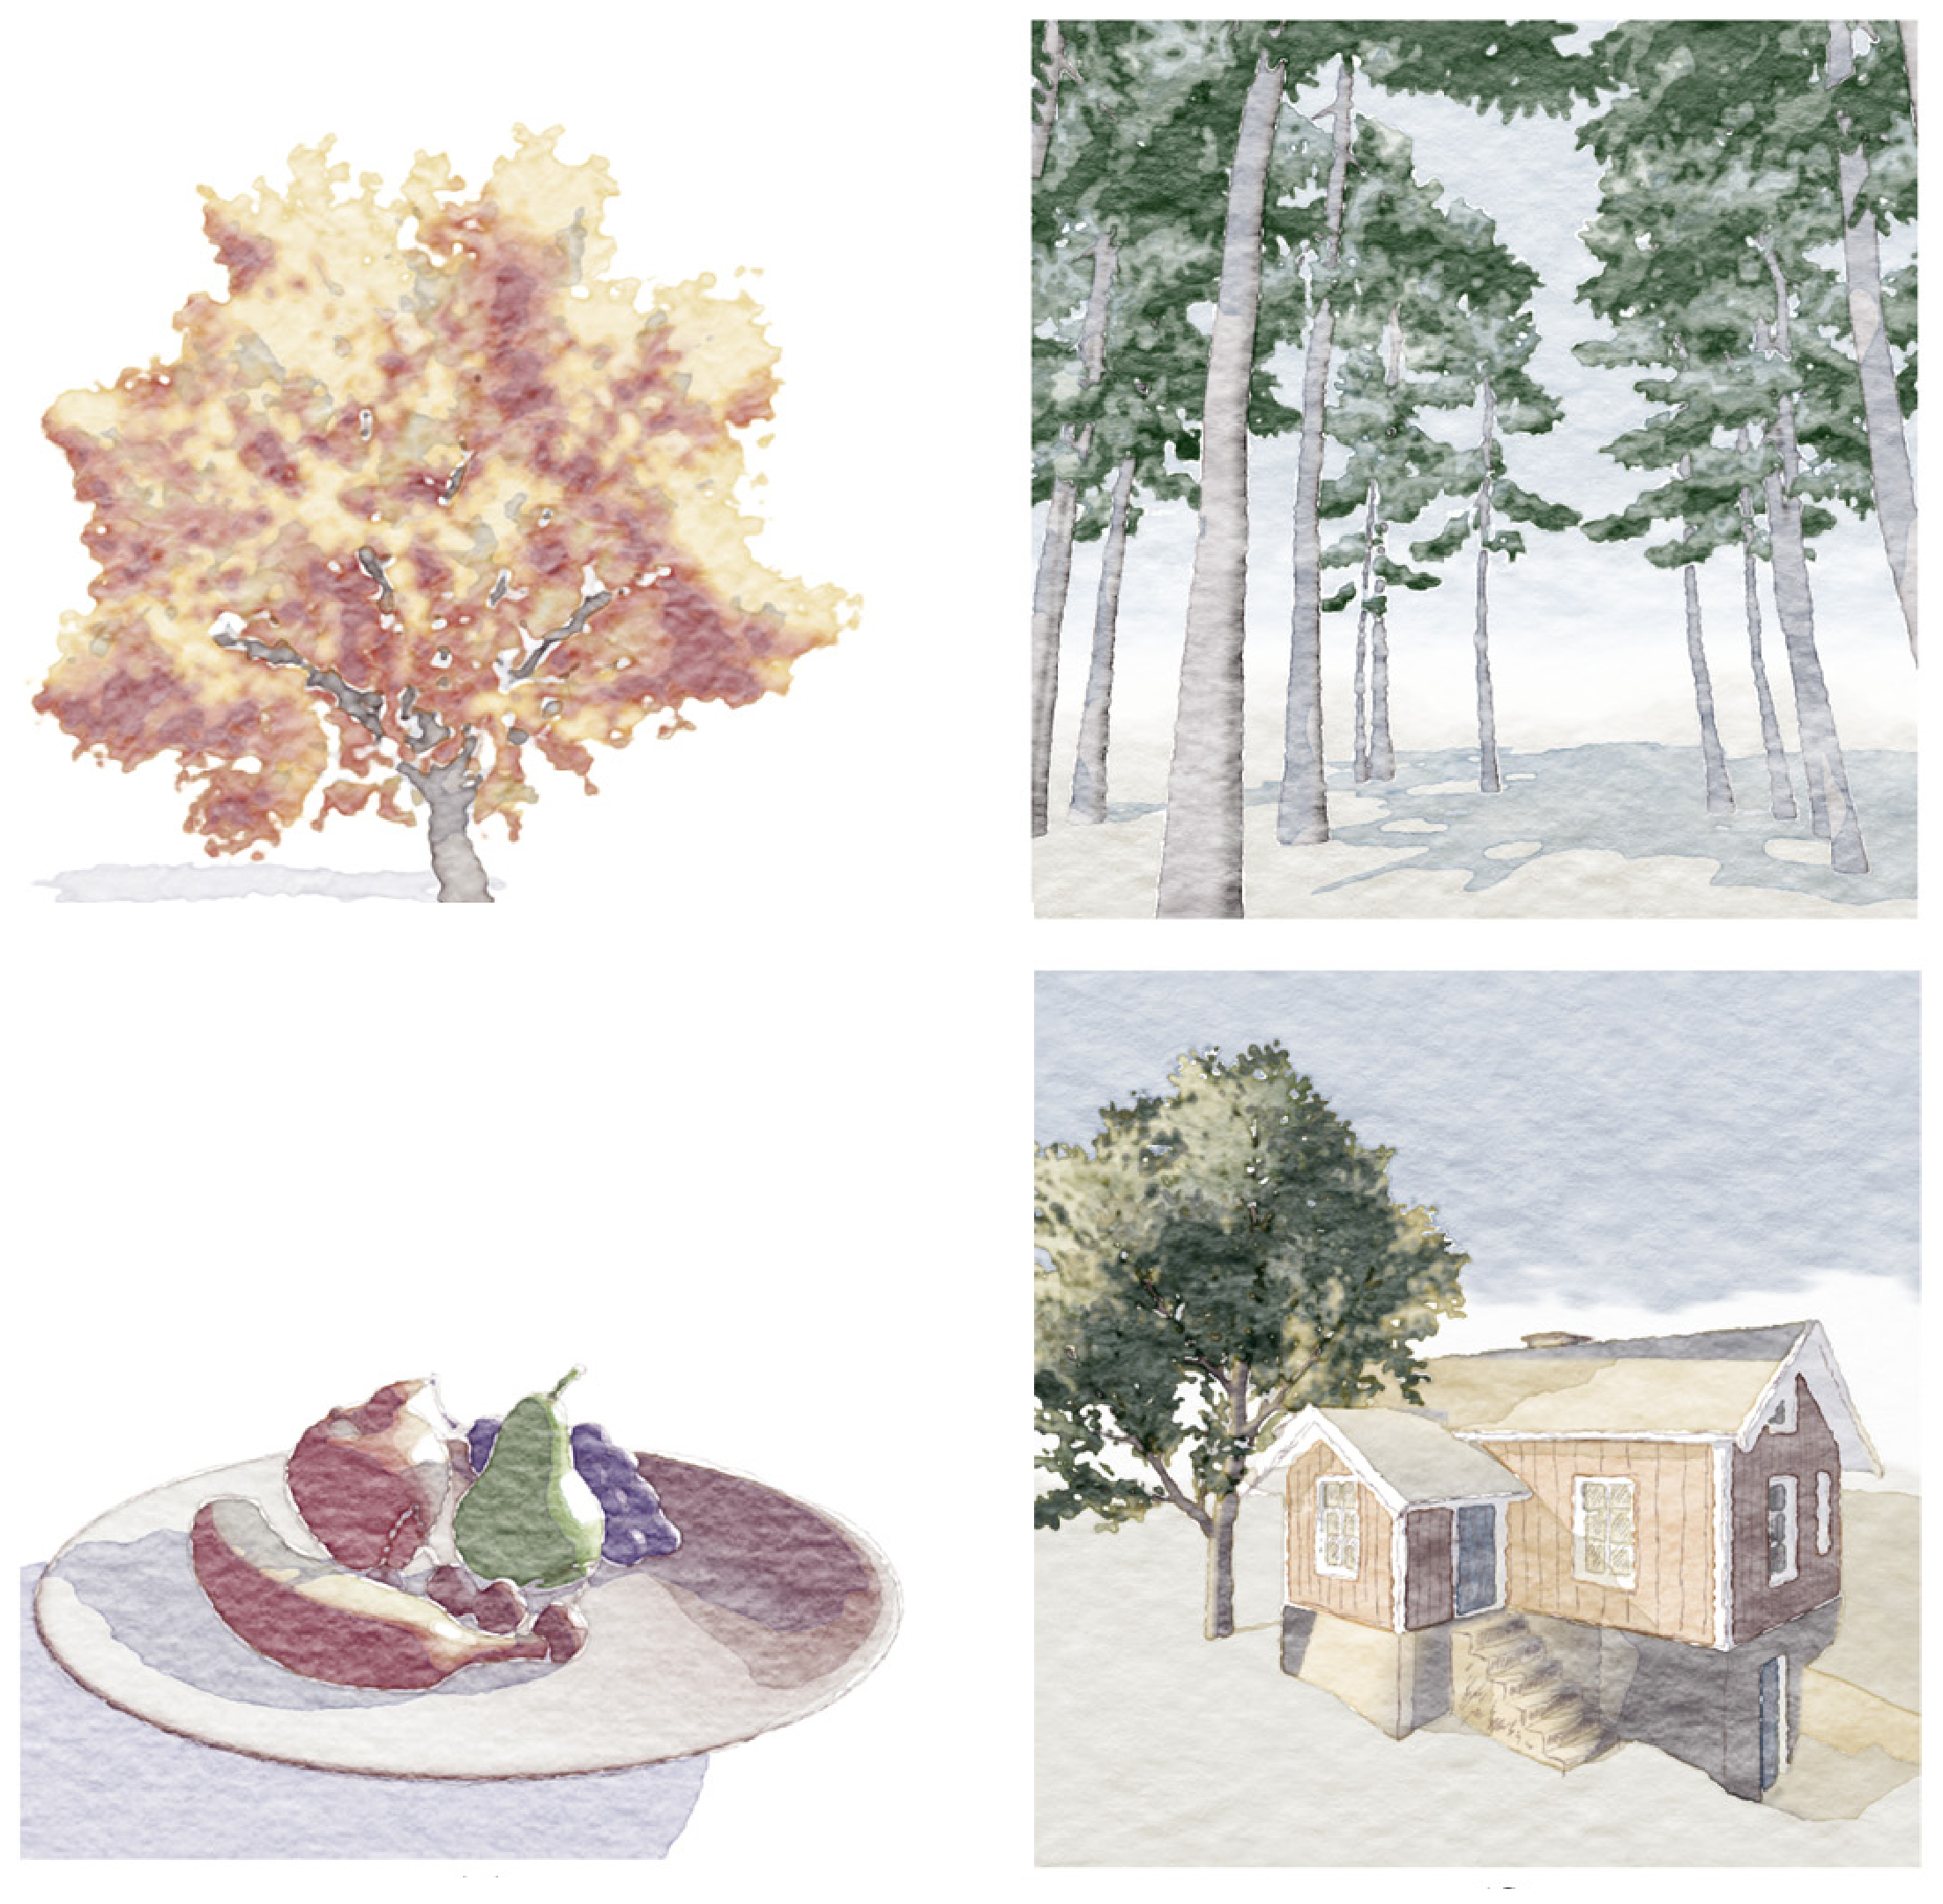
\includegraphics[width=0.8\textwidth]{../images/Luft2006-examples}
  \caption{Beispielbilder aus der Echtzeitanimation. Quelle: \cite{Luft2006}.}
  \label{fig:wcolor-results}
\end{figure}